\section*{Đề thi thử THPTQG Sở GD\&ĐT Bắc Ninh 25--26, Lần 2}


\Opensolutionfile{ans}[ans/ans 57-26-2--BacNinh-SoGD-L1-LC]

\caulc

\begin{ex} %Câu 1. %[1H8N2-2]
	\immini[thm]{Cho hình chóp $S.ABCD$ có đáy $ABCD$ là hình chữ nhật, đường thẳng $SA$ vuông góc với mặt phẳng $(ABCD)$. Đường thẳng $CD$ vuông góc với mặt phẳng nào dưới đây?
		\choice
		{$(SAC)$}
		{\True $(SAD)$}
		{$(SBC)$}
		{$(SAB)$}
	}{		\begin{tikzpicture}[scale=0.7, >=stealth]
			\coordinate (A) at (0,0);
			\coordinate (B) at (-1.5,-1.2);
			\coordinate (C) at (2.5,-1.2);
			\coordinate (D) at ($(A)+(C)-(B)$);
			\coordinate (S) at (0,2.8);
			\draw[dashed] (S)--(A)--(D) (A)--(B);
			\draw (S)--(B)--(C)--(D)--(S)--(C);
			\foreach \p/\pos in {S/above, A/above left, B/below left, C/below right, D/right} 
			\filldraw (\p) circle (1pt) node[\pos] {$\p$};
	\end{tikzpicture}}
	\loigiai{
		Ta có $\heva{&CD \perp AD \\ &CD \perp SA} \Rightarrow CD \perp (SAD).$
	}
\end{ex}


\begin{ex} %Câu 2. %[1D6H3-3]
	Tập hợp nghiệm của bất phương trình $\log_{0{,}5} x > -1$ là
	\choice
	{\True $(0;2)$}
	{$(-\infty;2)$}
	{$(0;+\infty)$}
	{$(2;+\infty)$}
	\loigiai{
		ĐKXĐ: $x > 0$. 
		
		BPT $\Leftrightarrow x < 0{,}5^{-1} \Leftrightarrow x < 2 $.
		Vậy $S = (0;2).$
		
		\textit{Lưu ý:} Khi giải bất phương trình lôgarit dạng $\log_a x > b$, học sinh cần đặc biệt chú ý hai vấn đề sau:
		\begin{itemize}
			\item \textbf{Điều kiện xác định:} Luôn phải đặt điều kiện cho biểu thức dưới dấu lôgarit dương ($x > 0$). Đây là bước dễ bị bỏ sót dẫn đến việc chọn nhầm đáp án $(-\infty; 2)$.
			\item \textbf{Cơ số $a$:} 
			\begin{itemize}
				\item Nếu $a > 1$: Bất phương trình giữ nguyên chiều.
				\item Nếu $0 < a < 1$: Bất phương trình phải \textbf{đổi chiều}. Trong bài toán này, cơ số\\ $a = 0{,}5 < 1$ nên từ $\log_{0{,}5} x > -1$ ta phải đổi chiều thành $x < 0{,}5^{-1}$.
			\end{itemize}
			\item Kết hợp điều kiện $x > 0$ và $x < 2$, ta được tập nghiệm chính xác là $(0; 2)$.
		\end{itemize}
	}
\end{ex}

\begin{ex} %Câu 3. %[2D1N4-1]
	Tiệm cận đứng của đồ thị hàm số $y = \dfrac{2x-3}{x+1}$ là đường thẳng có phương trình
	\choice
	{$x=2$}
	{$y=-1$}
	{$y=2$}
	{\True $x=-1$}
	\loigiai{
		Tập xác định của hàm số là $D = \mathbb{R} \setminus \{-1\}$.\\
		Ta có $\lim\limits_{x \to -1^+} \dfrac{2x-3}{x+1} = -\infty$ và $\lim\limits_{x \to -1^-} \dfrac{2x-3}{x+1} = +\infty$.\\
		Vậy đường thẳng $x = -1$ là tiệm cận đứng của đồ thị hàm số.
	}
\end{ex}

\begin{ex}%Câu 4. %[2H2N1-2]
	\immini[thm]{Cho hình hộp $ABCD.A'B'C'D'$. Vectơ $\overrightarrow{BA} + \overrightarrow{BC} + \overrightarrow{BB'}$ bằng vectơ nào dưới đây?
		\choice
		{\True $\overrightarrow{BD'}$}
		{$\overrightarrow{BC'}$}
		{$\overrightarrow{BA'}$}
		{$\overrightarrow{BD}$}
	}{
		\begin{tikzpicture}[scale=0.8, line join=round, line cap=round, >=stealth]
			% Tọa độ các đỉnh đáy dưới
			\coordinate (A) at (0,0);
			\coordinate (B) at (2.5,0);
			\coordinate (D) at (1.2,1);
			\coordinate (C) at ($(B)+(D)-(A)$);
			
			% Tọa độ các đỉnh đáy trên
			\coordinate (A1) at (0.5,2.5);
			\coordinate (B1) at ($(B)+(A1)-(A)$);
			\coordinate (D1) at ($(D)+(A1)-(A)$);
			\coordinate (C1) at ($(C)+(A1)-(A)$);
			
			% Vẽ các cạnh khuất
			\draw[dashed] (D1)--(D)--(A) (D)--(C);
			
			% Vẽ các cạnh thấy
			\draw (A)--(B)--(C)--(C1)--(D1)--(A1)--cycle;
			\draw (B)--(B1)--(C1) (B1)--(A1);
			
			% Vẽ vectơ minh họa (nếu cần nhấn mạnh)
			\draw[] (B)--(A);
			\draw[] (B)--(C);
			\draw[] (B)--(B1);
			%		\draw[] (B)--(D1);
			
			% Gán nhãn các đỉnh
			\node[left] at (A) {$A$};
			\node[below] at (B) {$B$};
			\node[right] at (C) {$C$};
			\node[above left] at (D) {$D$};
			\node[left] at (A1) {$A'$};
			\node[below right] at (B1) {$B'$};
			\node[right] at (C1) {$C'$};
			\node[above] at (D1) {$D'$};
			
			% Đánh dấu các điểm
			\foreach \p in {A,B,C,D,A1,B1,C1,D1}
			\fill (\p) circle (1.5pt);
		\end{tikzpicture}
	}
	\loigiai{
		\begin{center}
			\begin{tikzpicture}[scale=1, line join=round, line cap=round, >=stealth]
				% Tọa độ các đỉnh đáy dưới
				\coordinate (A) at (0,0);
				\coordinate (B) at (2.5,0);
				\coordinate (D) at (1.2,1);
				\coordinate (C) at ($(B)+(D)-(A)$);
				
				% Tọa độ các đỉnh đáy trên
				\coordinate (A1) at (0.5,2.5);
				\coordinate (B1) at ($(B)+(A1)-(A)$);
				\coordinate (D1) at ($(D)+(A1)-(A)$);
				\coordinate (C1) at ($(C)+(A1)-(A)$);
				
				% Vẽ các cạnh khuất
				\draw[dashed] (D1)--(D)--(A) (D)--(C);
				
				% Vẽ các cạnh thấy
				\draw (A)--(B)--(C)--(C1)--(D1)--(A1)--cycle;
				\draw (B)--(B1)--(C1) (B1)--(A1);
				
				% Vẽ vectơ minh họa (nếu cần nhấn mạnh)
				\draw[->,blue,thick] (B)--(A);
				\draw[->,blue,thick] (B)--(C);
				\draw[->,blue,thick] (B)--(B1);
				\draw[->,red,ultra thick, dashed] (B)--(D1);
				
				% Gán nhãn các đỉnh
				\node[left] at (A) {$A$};
				\node[below] at (B) {$B$};
				\node[right] at (C) {$C$};
				\node[above left] at (D) {$D$};
				\node[left] at (A1) {$A'$};
				\node[below right] at (B1) {$B'$};
				\node[right] at (C1) {$C'$};
				\node[above] at (D1) {$D'$};
				
				% Đánh dấu các điểm
				\foreach \p in {A,B,C,D,A1,B1,C1,D1}
				\fill (\p) circle (1.5pt);
			\end{tikzpicture}
		\end{center}
		Áp dụng quy tắc hình bình hành cho đáy $ABCD$, ta có $\overrightarrow{BA} + \overrightarrow{BC} = \overrightarrow{BD}$.\\
		Áp dụng quy tắc hình bình hành cho mặt $BDD'B'$, ta có $\overrightarrow{BD} + \overrightarrow{BB'} = \overrightarrow{BD'}$.\\
		Vậy $\overrightarrow{BA} + \overrightarrow{BC} + \overrightarrow{BB'} = \overrightarrow{BD'}$.
	}
\end{ex}

\begin{ex}%Câu 5. %[2D1N1-2]
	\immini[thm]{Cho hàm số bậc ba $y=f(x)$ có đồ thị là đường cong như hình vẽ.
		Hàm số đã cho đồng biến trên khoảng nào dưới đây?
		\choice
		{\True $(1;+\infty)$}
		{$(-1;1)$}
		{$(-1;+\infty)$}
		{$(-\infty;0)$}
	}{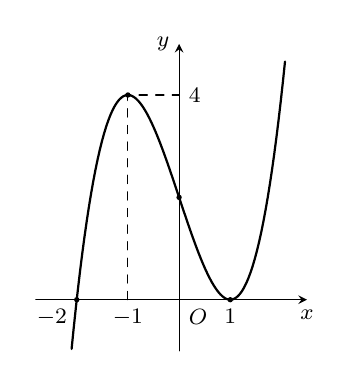
\begin{tikzpicture}[scale=0.65, font=\footnotesize, line join=round, line cap=round, >=stealth]
			% Vẽ trục tọa độ
			\draw[->] (-2.8,0) -- (2.5,0) node[below] {$x$};
			\draw[->] (0,-1) -- (0,5) node[left] {$y$};
			\node[below right] at (0,0) {$O$};
			
			% Vẽ đồ thị hàm bậc ba (mô phỏng theo image_d81604.png)
			% Hàm số mẫu: y = x^3 - 3x + 2
			\draw[thick, samples=100, domain=-2.1:2.07] plot (\x, {(\x)^3 - 3*(\x) + 2});
			
			% Vẽ các đường gióng và nhãn điểm
			\draw[dashed] (-1,0) node[below] {$-1$} -- (-1,4) -- (0,4) node[right] {$4$};
			\draw[dashed] (1,0) -- (1,0);
			\node[below] at (1,0) {$1$};
			\node[below left] at (-2,0) {$-2$};
			
			% Đánh dấu các điểm quan trọng
			\fill (-1,4) circle (1.5pt);
			\fill (1,0) circle (1.5pt);
			\fill (0,2) circle (1.5pt);
			\fill (-2,0) circle (1.5pt);
	\end{tikzpicture}}
	\loigiai{
		Dựa vào đồ thị, ta thấy đồ thị hàm số đi lên trên các khoảng $(-\infty; -1)$ và $(1; +\infty)$.\\
		Do đó, hàm số đồng biến trên các khoảng $(-\infty; -1)$ và $(1; +\infty)$.\\
		Đối chiếu với các phương án lựa chọn, ta chọn khoảng $(1; +\infty)$.
	}
\end{ex}




\begin{ex}%Câu 6. %[2H5N2-2]
	Trong không gian $Oxyz$, cho đường thẳng $\Delta$ có phương trình $\dfrac{x-1}{2} = \dfrac{y+2}{1} = \dfrac{z-4}{-3}$. Một vectơ chỉ phương của $\Delta$ có tọa độ là
	\choice
	{$(2;1;3)$}
	{$(1;2;4)$}
	{$(1;-2;4)$}
	{\True $(2;1;-3)$}
	\loigiai{
		Đường thẳng $\Delta \colon \dfrac{x-x_0}{a} = \dfrac{y-y_0}{b} = \dfrac{z-z_0}{c}$ có một vectơ chỉ phương là $\vec{u} = (a; b; c)$.\\
		Từ phương trình của $\Delta$ ta suy ra một vectơ chỉ phương là $\vec{u} = (2; 1; -3)$.
	}
\end{ex}

\begin{ex}%Câu 7. %[2D4N1-1]
	Họ nguyên hàm của hàm số $f(x) = 3\cos x$ trên $(-\infty;+\infty)$ là
	\choice
	{$-3\cos x + C$}
	{\True $3\sin x + C$}
	{$-3\sin x + C$}
	{$3\cos x + C$}
	\loigiai{
		Ta có $\displaystyle\int \cos x \, \text{d}x = 3\sin x + C$.
	}
\end{ex}


\begin{ex}%Câu 8. %[2H5N1-3]
	Trong không gian $Oxyz$, cho điểm $M(1;2;3)$ và mặt phẳng $(P) \colon x + 3y - 4z + 9 = 0$. Mặt phẳng $(Q)$ đi qua $M$ và song song với $(P)$ có phương trình là
	\choice
	{$x + 3y + 4z + 5 = 0$}
	{$x + 3y - 4z + 6 = 0$}
	{\True $x + 3y - 4z + 5 = 0$}
	{$x + 3y - 4z - 5 = 0$} 
	\loigiai{
		Mặt phẳng $(Q) \parallel (P)$ nên $(Q)$ có dạng: $x + 3y - 4z + D = 0$ ($D \neq 9$).\\
		Vì $M(1;2;3) \in (Q)$ nên: $1 + 3(2) - 4(3) + D = 0 \Leftrightarrow D = 5$.\\
		Vậy phương trình $(Q)$ là $x + 3y - 4z + 5 = 0$.
	}
\end{ex}

\begin{ex}%Câu 9. %[2D4N2-1]
	Biết $F(x) = \dfrac{1}{x}$ là một nguyên hàm của hàm số $f(x)$ trên $(0;+\infty)$. Giá trị của $\displaystyle\int_1^3 6[f(x) + x] \, \text{d}x$ bằng
	\choice
	{$6\ln 2 + 24$}
	{$28$}
	{\True $20$}
	{$\ln 3 + 24$}
	\loigiai{
		Ta có $$\displaystyle\int_1^3 6[f(x) + x] \, \text{d}x = 6 \cdot F(x) \Big|_1^3 + 6 \cdot \dfrac{x^2}{2} \Big|_1^3 = 20.$$
	}
\end{ex}


\begin{ex}%Câu 10. %[2D1N2-2]
	Cho hàm số $y = f(x) = \dfrac{mx^2+nx+p}{qx+r}$ có bảng biến thiên như hình vẽ.
	
	\begin{center}
		%!<\usepackage{tkz-tab}>
		
		
\begin{tikzpicture}[line cap=round, line join=round, >=stealth, font=\footnotesize]
			% Sử dụng tkz-tab để vẽ bảng biến thiên dựa trên hình ảnh image_70e1fe.png
			% Các điểm đặc biệt: cực đại tại x = -1, cực tiểu tại x = 3, tiệm cận đứng tại x = 1
			
			\tkzTabInit[lgt=1.5, espcl=2.5]
			{$x$ / 1, $f'(x)$ / 1, $f(x)$ / 2.5}
			{$-\infty$, $-1$, $1$, $3$, $+\infty$}
			
			% Dòng đạo hàm: dương, không, âm, không xác định (t), âm, không, dương
			\tkzTabLine{, +, z, -, d, -, z, +, }
			
			% Dòng biến thiên:
			% Nhánh 1: Tăng từ -vô cùng lên -4, giảm xuống -vô cùng tại tiệm cận đứng x = 1
			% Nhánh 2: Giảm từ +vô cùng xuống 4 tại x = 3, tăng lên +vô cùng
			\tkzTabVar{-/$-\infty$, +/$-4$, -D+/$-\infty$/$+\infty$, -/$4$, +/$+\infty$}
			
		\end{tikzpicture}
	\end{center}
	
	Giá trị cực tiểu của hàm số đã cho bằng
	\choice
	{$-4$}
	{$3$}
	{\True $4$}
	{$-1$}
	\loigiai{
		Dựa vào bảng biến thiên, hàm số đạt cực tiểu tại $x=3$ và giá trị cực tiểu tương ứng là $f(3) = 4$.
	}
\end{ex}

\begin{ex}%Câu 11. %[1D2H2-4]
	Cho cấp số cộng $(u_n)$ có $u_2 = 4, u_3 = 2$. Khẳng định nào sau đây là đúng?
	\choice
	{\True $u_1 = 6$}
	{$u_1 = 0$}
	{$u_1 = 8$}
	{$u_1 = 2$}
	\loigiai{
		Công sai $d = u_3 - u_2 = 2 - 4 = -2$.\\
		Ta có $u_2 = u_1 + d \Rightarrow u_1 = u_2 - d = 4 - (-2) = 6$.
	}
\end{ex}

\begin{ex}%Câu 12. %[1D5N1-4]
	Xét mẫu số liệu cho bởi bảng ghép nhóm sau đây:
	\begin{center}
		\begin{tabular}{|c|c|c|c|c|c|}
			\hline
			Nhóm & $[0;4)$ & $[4;8)$ & $[8;12)$ & $[12;16)$ & $[16;20)$ \\ \hline
			Tần số & $6$ & $12$ & $14$ & $8$ & $5$ \\ \hline
		\end{tabular}
	\end{center}
	Nhóm chứa mốt của mẫu số liệu trên là
	\choice
	{\True $[8;12)$}
	{$[16;20)$}
	{$[12;16)$}
	{$[4;8)$}
	\loigiai{
		Nhóm chứa mốt là nhóm có tần số lớn nhất. Trong bảng trên, tần số lớn nhất là $14$ tương ứng với nhóm $[8;12)$.
	}
\end{ex}

\cauds
\Opensolutionfile{ans}[ans/ans 57-26-2--BacNinh-SoGD-L1-DS]
\begin{ex}%Câu 1. %[2D6V2-3]
	Một hộp có chứa $9$ quả bóng màu xanh và $16$ quả bóng màu đỏ (các quả bóng có cùng hình dạng, kích thước và khối lượng). Bạn Nguyệt lấy ngẫu nhiên một quả bóng từ hộp đó (không trả lại). Nếu bạn Nguyệt lấy được quả bóng màu xanh thì bạn Đức lấy ngẫu nhiên đồng thời hai quả bóng từ số bóng còn lại trong hộp. Nếu bạn Nguyệt lấy được quả bóng màu đỏ thì bạn Đức lấy ngẫu nhiên đồng thời ba quả bóng từ số bóng còn lại trong hộp.
	\choiceTFt
	{Xác suất để bạn Nguyệt lấy được quả bóng màu xanh là $0{,}4$}
	{Nếu bạn Nguyệt lấy được quả bóng màu xanh thì xác suất để bạn Đức lấy được ít nhất một quả bóng màu đỏ là $0{,}46$ \textit{(kết quả làm tròn đến hàng phần trăm})}
	{\True Nếu bạn Nguyệt lấy được quả bóng màu đỏ thì xác suất để bạn Đức lấy được ít nhất một quả bóng màu xanh là $0{,}78$ (\textit{kết quả làm tròn đến hàng phần trăm})}
	{\True Biết rằng trong tất cả các quả bóng hai bạn Nguyệt và Đức lấy ra có đủ cả bóng màu xanh và bóng màu đỏ, thì xác suất để bạn Nguyệt lấy được quả bóng màu xanh là $0{,}39$ (\textit{kết quả làm tròn đến hàng phần trăm})}
	\loigiai{
		
		Gọi $A$ là biến cố "Nguyệt lấy được bóng xanh" $\Rightarrow P(A) = \dfrac{9}{25}=0{,}36$ và $P(\overline{A}) = 0{,}64$. \\
		Gọi $B$ là biến cố "Đức lấy được ít nhất một quả bóng màu xanh".
		
		\begin{center}
			\begin{tikzpicture}[
				grow=right,
				level 1/.style={sibling distance=3.5cm, level distance=5.5cm},
				level 2/.style={sibling distance=1.8cm, level distance=5cm},
				edge from parent/.style={draw, -latex, thick},
				sloped, font=\small
				]
				\node[circle, draw] {$\Omega$}
				child {
					node[red] {Nguyệt Đỏ ($\overline{A}$)}
					child { node {Đức $0$ Xanh } edge from parent node[below] {$\approx 0{,}22$} }
					child { node {Đức $\ge 1$ Xanh } edge from parent node[above] {$\approx 0{,}78$} }
					edge from parent node[below] {$0{,}64$}
				}
				child {
					node[blue] {Nguyệt Xanh ($A$)}
					child { node {Đức $0$ Đỏ} edge from parent node[below] {$\approx 0{,}10$} }
					child { node {Đức $\ge 1$ Đỏ} edge from parent node[above] {$\approx 0{,}90$} }
					edge from parent node[above] {$0{,}36$}
				};
			\end{tikzpicture}
		\end{center}
		\begin{itemchoice}
			\itemch \textbf{Sai.} $P(A) = 0{,}36$.
			\itemch \textbf{Sai.} Khi $A$ xảy ra, Đức lấy $2$ quả từ $24$ quả ($8$ xanh, $16$ đỏ). \\
			Xác suất Đức lấy ít nhất $1$ quả đỏ là:
			$$P(\text{Đức } \ge 1 \text{ Đỏ}|A) = 1 - \dfrac{\mathrm{C}_8^2}{\mathrm{C}_{24}^2} = \dfrac{62}{69} \approx 0{,}90.$$
			\itemch \textbf{Đúng.} Khi $\overline{A}$ xảy ra, Đức lấy $3$ quả từ $24$ quả ($9$ xanh, $15$ đỏ). \\
			Xác suất Đức lấy ít nhất $1$ quả xanh là:
			$$P(\text{Đức } \ge 1 \text{ Xanh}|\overline{A}) = 1 - \dfrac{\mathrm{C}_{15}^3}{\mathrm{C}_{24}^3} = \dfrac{1569}{2024} \approx 0{,}78.$$
			\itemch \textbf{Đúng.} Gọi $H$ là biến cố Đức lấy được quả có đủ hai màu. \\
			Áp dụng công thức xác suất đầy đủ, ta có:
			$$P(H) = P(A) \cdot P(\text{Đức } \ge 1 \text{ Đỏ}|A) + P(\overline{A}) \cdot P(\text{Đức } \ge 1 \text{ Xanh}|\overline{A}) \approx 0{,}8196.$$
			Xác suất cần tìm áp dụng công thức Bayes là:
			$$P(A|H) = \dfrac{P(A \cap H)}{P(H)} = \dfrac{0{,}36 \cdot \dfrac{62}{69}}{0{,}8196} \approx 0{,}39.$$
		\end{itemchoice}
	}
\end{ex}
\begin{ex} %Câu 2. %[2D1V3-6]
	Cho hàm số $y = f(x) = \dfrac{3x + 2}{x - 1}$ có đồ thị là $(C)$ và hai điểm $A(-4; 2)$, $B(2; 8)$.
	\choiceTFt
	{\True $\forall x \neq 1$, hàm số đã cho có đạo hàm $y' = \dfrac{-5}{(x - 1)^2}$}
	{Tâm đối xứng của đồ thị hàm số đã cho là điểm $I(3; 1)$}
	{\True Gọi $m, M$ lần lượt là giá trị nhỏ nhất, giá trị lớn nhất của hàm số $y = f(x)$ trên $[2; 5]$. Khi đó $4m + M = 25$}
	{\True Điểm $K(a; b) \in (C)$ sao cho trực tâm $H$ của tam giác $KAB$ thuộc vào đường thẳng $d: 5x + 4y + 3 = 0$. Khi đó, giá trị của biểu thức $4a^2 - 3b$ bằng $6$}
	\loigiai{
		Xét hàm số $y = \dfrac{3x+2}{x-1}$ trên tập xác định $D = \mathbb{R} \setminus \{1\}$.
		\begin{itemchoice}
			\itemch \textbf{Đúng.} Áp dụng công thức đạo hàm hàm phân thức bậc nhất: 
			$$y' = \dfrac{3(-1) - 2(1)}{(x-1)^2} = \dfrac{-5}{(x-1)^2}.$$
			
			\itemch \textbf{Sai.} Tiệm cận đứng là $x=1$, tiệm cận ngang là $y=3$. Tâm đối xứng của đồ thị là giao điểm hai đường tiệm cận, có tọa độ là $(1; 3)$, không phải $(3; 1)$.
			
			\itemch \textbf{Đúng.} Vì $y' < 0$ với mọi $x \in D$ nên hàm số nghịch biến trên $[2; 5]$.\\
			Do đó $M = f(2) = 8$ và $m = f(5) =  4{,}25$.\\
			Ta có $4m + M = 4 \cdot \dfrac{17}{4} + 8 = 25$. 
			
			\itemch \textbf{Đúng.} Nhận xét: $A(-4; 2) \in (C)$ và $B(2; 8) \in (C)$. Do $K, A, B$ cùng thuộc đồ thị hàm phân thức bậc nhất $(C)$ nên trực tâm $H$ của tam giác $KAB$ cũng thuộc $(C)$. \\
			Mặt khác $H \in d: 5x + 4y + 3 = 0$, tọa độ $H$ là nghiệm của hệ:
			$$\heva{&y = \dfrac{3x+2}{x-1} \\ &5x + 4y + 3 = 0}  \Rightarrow H\left(-1; \dfrac{1}{2}\right).$$
			Với $\overrightarrow{AH} = (3; -1{,}5)$ và $\overrightarrow{BK} = (a-2; b-8)$, ta có:
			
			$$\vec{AH}.\vec{BK}=0 \Leftrightarrow
			3(a-2) - 1{,}5(b-8) = 0 \Leftrightarrow b = 2a + 4.$$
			Thay $b = 2a + 4$ vào phương trình  $y = 3 + \dfrac{5}{x-1}$, ta được:
			$$2a + 4 = 3 + \dfrac{5}{a-1} \Leftrightarrow 2a^2 - a - 6 = 0 \Leftrightarrow \hoac{&a = 2 \text{ (loại vì } K \equiv B) \\ &a = -1{,}5}$$
			Với $a = -1{,}5 \Rightarrow b = 1$. Vậy $4a^2 - 3b = 6$.
		\end{itemchoice}
		
	}
\end{ex}
\begin{ex}%Câu 3. %[2H5V2-7]
	Trong không gian $Oxyz$, cho hai điểm $A(2; 4; 1)$, $B(-2; 2; -3)$ và mặt phẳng $(P) \colon x + y + z - 3 = 0$.
	\choiceTF
	{Phương trình mặt phẳng trung trực của đoạn thẳng $AB$ là $2x + y + 2z + 1 = 0$}
	{\True Toạ độ trung điểm $I$ của đoạn thẳng $AB$ là $(0; 3; -1)$}
	{\True Phương trình mặt cầu đường kính $AB$ là $x^2 + (y - 3)^2 + (z + 1)^2 = 9$}
	{\True Gọi $M$ là điểm di động trên mặt phẳng $(P)$ sao cho $M$ luôn cách đều hai điểm $A$ và $B$. Khoảng cách ngắn nhất từ $M$ đến gốc toạ độ $O$ bằng $3\sqrt{3}$}
	\loigiai{
		\begin{itemchoice}
			\itemch \textbf{Sai.} \\
			Trung điểm của $AB$ là $I(0; 3; -1)$. \\
			Vectơ $\overrightarrow{AB} = (-4; -2; -4)$, chọn VTPT của mặt phẳng trung trực $(\alpha)$ là $\vec{n}_{\alpha} = (2; 1; 2)$. \\
			Phương trình $(\alpha) \colon 2(x - 0) + 1(y - 3) + 2(z + 1) = 0 \Leftrightarrow 2x + y + 2z - 1 = 0$.
			
			\itemch \textbf{Đúng.} \\
			Toạ độ trung điểm $I$ của $AB$: $x_I = \dfrac{2-2}{2} = 0$; $y_I = \dfrac{4+2}{2} = 3$; $z_I = \dfrac{1-3}{2} = -1$. \\
			Vậy $I(0; 3; -1)$.
			
			\itemch \textbf{Đúng.} \\
			Mặt cầu đường kính $AB$ có tâm $I(0; 3; -1)$, bán kính: $R = \dfrac{AB}{2} = \dfrac{6}{2} = 3.$
			
			Phương trình mặt cầu: $x^2 + (y - 3)^2 + (z + 1)^2 = 9$.
			
			\itemch \textbf{Đúng.} \\
			$M$ cách đều $A, B \Rightarrow M \in (\alpha) \colon 2x + y + 2z - 1 = 0$. \\
			Mà $M \in (P) \colon x + y + z - 3 = 0$ nên $M$ thuộc đường thẳng $\Delta$ là giao tuyến của $(\alpha)$ và $(P)$. \\
			Đường thẳng $\Delta$ có VTCP $\vec{u}_{\Delta} = [\vec{n}_{\alpha}, \vec{n}_P] = (-1; 0; 1)$ và đi qua $N(-2; 5; 0)$. \\
			Khoảng cách ngắn nhất từ $O$ đến $M$ là $OM_{\min} = d(O, \Delta) = \dfrac{|[\overrightarrow{ON}, \vec{u}_{\Delta}]|}{|\vec{u}_{\Delta}|}$. \\
			Ta có $\overrightarrow{ON} = (-2; 5; 0) \Rightarrow [\overrightarrow{ON}, \vec{u}_{\Delta}] = (5; 2; 5)$. \\
			$$\Rightarrow OM_{\min} = \dfrac{\sqrt{5^2 + 2^2 + 5^2}}{\sqrt{(-1)^2 + 0^2 + 1^2}}  = 3\sqrt{3}.$$
			\textit{Lưu ý:} Ngoài cách tính khoảng cách trực tiếp, ta có thể sử dụng phương pháp hàm số: \\
			Đường thẳng $\Delta$ đi qua $N(-2; 5; 0)$ và có VTCP $\vec{u} = (-1; 0; 1)$ có phương trình tham số:
			$$\Delta: \heva{&x = -2 - t \\ &y = 5 \\ &z = t} (t \in \mathbb{R}).$$
			Vì $M \in \Delta$ nên  $M(-2-t; 5; t)$. Khi đó:
			$$OM^2 = (-2-t)^2 + 5^2 + t^2 = 2t^2 + 4t + 29.$$
			Ta có $OM^2 = 2(t + 1)^2 + 27 \ge 27, \forall t \in \mathbb{R}$. \\
			Suy ra $OM_{\min} = \sqrt{27} = 3\sqrt{3}$ khi $t = -1$.
		\end{itemchoice}
		
	}
\end{ex}
\begin{ex}%Câu 4. %[2D4V2-6]
	Trong một bể xử lý nước thải, số lượng vi khuẩn gây hại tại thời điểm $t$ được kí hiệu bằng $N(t)$ (đơn vị: con). Người ta nhận thấy rằng trong giai đoạn đầu (khi môi trường chưa bị hạn chế), tốc độ biến thiên của số lượng vi khuẩn tuân theo quy luật hàm mũ và được mô hình hóa bởi hàm số $N'(t) = A \cdot \mathrm{e}^{kt}$, trong đó: $A, k$ là các hằng số dương, $t$ là thời gian (đơn vị: giờ). Từ các nghiên cứu thực nghiệm (sau khi xử lý và làm tròn số liệu), người ta ước lượng được $A = 1000\ln 2$ và tại thời điểm $t=1$ giờ có $3000$ vi khuẩn; $N'(1) = 2000 \ln 2$. Biết rằng mức độ an toàn cho phép là không quá $129\,000$ con.
	\choiceTF
	{\True $k = \ln 2$}
	{Số vi khuẩn tại thời điểm $t=6$ giờ là $63\,000$ con}
	{\True Số lượng vi khuẩn bắt đầu vượt ngưỡng an toàn từ sau thời điểm $t=7$ giờ}
	{Tại thời điểm $t=7$ giờ người ta tiến hành xử lý để giảm số lượng vi khuẩn theo quy luật: $M(t) = 129\,000 \cdot \mathrm{e}^{-0{,}5(t-7)}$ với $M(t)$ là số con vi khuẩn ở thời điểm $t$ giờ ($t \ge 7$). Khi đó, sau $3\ln 2$ giờ kể từ khi bắt đầu xử lý, số vi khuẩn còn lại $64\,500$ con}
	\loigiai{
		\begin{itemchoice}
			\itemch \textbf{Đúng:} Ta có $N'(t) = 1000\ln 2 \cdot \mathrm{e}^{kt}$. \\
			Với $t=1$, $N'(1) = 1000\ln 2 \cdot \mathrm{e}^k = 2000\ln 2 \Rightarrow \mathrm{e}^k = 2 \Rightarrow k = \ln 2$.
			
			\itemch \textbf{Sai:} Ta có $N(t) = \displaystyle\int 1000\ln 2 \cdot \mathrm{e}^{t\ln 2} \mathrm{d}t = 1000 \cdot 2^t + C$. \\
			Vì $N(1) = 3000 \Rightarrow 1000 \cdot 2^1 + C = 3000 \Rightarrow C = 1000$. \\
			Do đó $N(t) = 1000 \cdot 2^t + 1000$. \\
			Tại $t=6$, $N(6) = 1000 \cdot 2^6 + 1000 = 65\,000 \neq 63\,000$.
			
			\itemch \textbf{Đúng:} Để $N(t) > 129\,000 \Leftrightarrow 1000 \cdot 2^t + 1000 > 129\,000 \Leftrightarrow 2^t > 128 \Leftrightarrow t > 7$.
			
			\itemch \textbf{Sai:} Sau $3\ln 2$ giờ kể từ khi bắt đầu xử lý ($t=7$), số vi khuẩn còn lại là: 
			$$M(7 + 3\ln 2) = 129\,000 \cdot \mathrm{e}^{-0{,}5(3\ln 2)} = 129\,000 \cdot 2^{-1{,}5} \approx 45\,608 \neq 64\,500.$$
		\end{itemchoice}
	}
\end{ex}
\caukq
\Opensolutionfile{ans}[ans/ans 57-26-2--BacNinh-SoGD-L1-KQ]
\begin{ex}%Câu 1. %[1H8V7-9]
	Cho hình chóp $S.ABCD$ có đáy $ABCD$ là hình chữ nhật với $AB = 2, AD = 2\sqrt{3}$, cạnh $SA$ vuông góc với mặt phẳng đáy $(ABCD)$. Biết khoảng cách từ $C$ đến mặt phẳng $(SBD)$ bằng $\dfrac{2\sqrt{15}}{5}$. Thể tích của khối chóp $S.ABCD$ bằng bao nhiêu?
	\shortans[oly]{8}
	\loigiai{
		\begin{center}
			\begin{tikzpicture}[scale=0.9, font=\footnotesize, line join=round, line cap=round, >=stealth]
				% Tọa độ các đỉnh
				\coordinate (A) at (0,0);
				\coordinate (B) at (-1,-2);
				\coordinate (D) at (4,0);
				\coordinate (C) at ($(B)+(D)-(A)$);
				\coordinate (S) at (0,3);
				\coordinate (O) at ($(A)!0.5!(C)$);
				
				% Xác định K trên BD sao cho AK vuông góc BD
				\coordinate (K) at ($(B)!0.4!(D)$);
				% Xác định H trên SK sao cho AH vuông góc SK
				\tkzDefPointBy[projection=onto S--K](A) \tkzGetPoint{H}
				
				% Vẽ các cạnh
				\draw[dashed] (S)--(A)--(D) (A)--(B) (A)--(C) (B)--(D) (A)--(K) (A)--(H) (S)--(K);
				\draw (S)--(B)--(C)--(D)--(S) (S)--(C) ;
				
				% Ký hiệu điểm
				\fill (A) circle (1.5pt) node[left] {$A$};
				\fill (B) circle (1.5pt) node[below] {$B$};
				\fill (C) circle (1.5pt) node[right] {$C$};
				\fill (D) circle (1.5pt) node[above right] {$D$};
				\fill (S) circle (1.5pt) node[above] {$S$};
				\fill (K) circle (1.5pt) node[below] {$K$};
				\fill (H) circle (1.5pt) node[right] {$H$};
				\fill (O) circle (1.5pt) node[below] {$O$};
				% Ký hiệu vuông góc
				\tkzMarkRightAngle[size=0.2](S,A,D)
				\tkzMarkRightAngle[size=0.2](A,K,D)
				\tkzMarkRightAngle[size=0.2](A,H,S)
			\end{tikzpicture}
		\end{center}
		
		Gọi $O = AC \cap BD$. Vì $O$ là trung điểm $AC$ nên $d(C, (SBD)) = d(A, (SBD)) = \dfrac{2\sqrt{15}}{5}$.
		
		Trong mặt phẳng $(ABCD)$, kẻ $AK \perp BD$ tại $K$. \\
		Ta có $BD \perp AK$ và $BD \perp SA$ (do $SA \perp (ABCD)$). \\
		$\Rightarrow BD \perp (SAK)$.
		
		Trong mặt phẳng $(SAK)$, kẻ $AH \perp SK$ tại $H$. \\
		Vì $BD \perp (SAK) \Rightarrow BD \perp AH$. \\
		Từ đó suy ra $AH \perp (SBD)$, do đó $AH = d(A, (SBD)) = \dfrac{2\sqrt{15}}{5}$.
		
		Xét tam giác vuông $ABD$ tại $A$:
		$$\dfrac{1}{AK^2} = \dfrac{1}{AB^2} + \dfrac{1}{AD^2} = \dfrac{1}{2^2} + \dfrac{1}{(2\sqrt{3})^2} =\dfrac{1}{3} \Rightarrow AK = \sqrt{3}.$$
		
		Xét tam giác vuông $SAK$ tại $A$:
		$$\dfrac{1}{AH^2} = \dfrac{1}{SA^2} + \dfrac{1}{AK^2} \Leftrightarrow \dfrac{25}{60} = \dfrac{1}{SA^2} + \dfrac{1}{3}  \Rightarrow SA = 2\sqrt{3}.$$
		
		Thể tích khối chóp $S.ABCD$ là: 
		$$V = \dfrac{1}{3} . SA. AB. AD = \dfrac{1}{3} .  2\sqrt{3}.2. 2\sqrt{3} = 8.$$
		
		\textit{Lưu ý:} Vì $SA, AB, AD$ đôi một vuông góc nên ta có thể dùng nhanh công thức cho tứ diện vuông $ASBD$: $\dfrac{1}{AH^2} = \dfrac{1}{SA^2} + \dfrac{1}{AB^2} + \dfrac{1}{AD^2}$.
		
		\textbf{Cách 2: Phương pháp tọa độ hóa} \\
		Chọn hệ trục tọa độ $Oxyz$ sao cho $A(0;0;0)$, $B(2;0;0)$, $D(0;2\sqrt{3};0)$ và $S(0;0;h)$ với $h > 0$.
		\begin{center}
			\begin{tikzpicture}[scale=1, font=\footnotesize, line join=round, line cap=round, >=stealth]
				% 1. Tọa độ các đỉnh (dựa trên AB=2, AD=2\sqrt{3})
				\coordinate (A) at (0,0);
				\coordinate (B) at (-2.5,-1); % Góc nhìn hệ trục
				\coordinate (D) at (4,0);
				\coordinate (C) at ($(B)+(D)-(A)$);
				\coordinate (S) at (0,3.5);
				
				% 2. Vẽ hệ trục tọa độ Oxyz gắn tại A (Nét đứt bên trong, nét liền bên ngoài)
				% Trục x: Đi qua B. Đoạn AB đứt, đoạn từ B ra ngoài liền.
				\draw[dashed, thick, red] (A) -- (B);
				\draw[->, thick, red] (B) -- ($(A)!1.4!(B)$) node[below] {$x$};
				
				% Trục y: Đi qua D. Đoạn AD đứt, đoạn từ D ra ngoài liền.
				\draw[dashed, thick, red] (A) -- (D);
				\draw[->, thick, red] (D) -- ($(A)!1.25!(D)$) node[below] {$y$};
				
				% Trục z: Đi qua S. Đoạn AS đứt, đoạn từ S ra ngoài liền.
				\draw[dashed, thick, red] (A) -- (S);
				\draw[->, thick, red] (S) -- ($(A)!1.15!(S)$) node[left] {$z$};
				
				\node[red, above left] at (A) {$A \equiv O$};
				
				% 3. Vẽ các cạnh của hình chóp (SA, AB, AD đã được vẽ đứt ở phần trục trục để trùng khít)
				\draw[dashed] (B)--(D);
				\draw[thick] (S)--(B)--(C)--(D)--(S) (S)--(C);
				
				% 4. Ký hiệu và nhãn các điểm
				\fill (A) circle (1.5pt);
				\fill (B) circle (1.5pt) node[below ] {$B$};
				\fill (C) circle (1.5pt) node[below right] {$C$};
				\fill (D) circle (1.5pt) node[below ] {$D$};
				\fill (S) circle (1.5pt) node[above left] {$S$};
				
				% Ký hiệu vuông góc tại gốc tọa độ trên các phẳng phẳng trục
				\draw[red, thin] (-0.25,-0.1) -- (-0.25,0.2) -- (0,0.3) -- (0.3,0.3) -- (0.3,0);
			\end{tikzpicture}
		\end{center}
		
		Khi đó ta có tọa độ các điểm: $C(2; 2\sqrt{3}; 0)$, $B(2; 0; 0)$, $D(0; 2\sqrt{3}; 0)$, $S(0; 0; h)$.
		
		Phương trình mặt phẳng $(SBD)$ có dạng mặt chắn:
		$$\dfrac{x}{2} + \dfrac{y}{2\sqrt{3}} + \dfrac{z}{h} = 1 \Leftrightarrow \sqrt{3}hx + hy + 2\sqrt{3}z - 2\sqrt{3}h = 0.$$
		
		Khoảng cách từ $C(2; 2\sqrt{3}; 0)$ đến mặt phẳng $(SBD)$:
		$$d(C, (SBD)) = \dfrac{\big|\sqrt{3}h(2) + h(2\sqrt{3}) + 2\sqrt{3}(0) - 2\sqrt{3}h\big|}{\sqrt{(\sqrt{3}h)^2 + h^2 + (2\sqrt{3})^2}} = \dfrac{2\sqrt{3}h}{\sqrt{4h^2 + 12}} = \dfrac{\sqrt{3}h}{\sqrt{h^2 + 3}}.$$
		
		Theo giả thiết $d(C, (SBD)) = \dfrac{2\sqrt{15}}{5}$, ta có phương trình:
		$$\dfrac{\sqrt{3}h}{\sqrt{h^2 + 3}} = \dfrac{2\sqrt{15}}{5}  \Leftrightarrow h^2 = 12 \Rightarrow h = 2\sqrt{3}.$$
		
		Thể tích khối chóp: $V = \dfrac{1}{3} . 2\sqrt{3} .2. 2\sqrt{3} = 8$.
		
	}
\end{ex}

\begin{ex}%Câu 2. %[2D1V5-8]
	\immini[thm]{Khi đặt trong mặt phẳng tọa độ $Oxy$ với trục $Ox$ nằm ngang trên mặt đất, trục $Oy$ hướng thẳng lên trên (tham khảo hình vẽ), đơn vị trong hệ trục là $1$ kilômét thì đường đi của một khinh khí cầu được mô phỏng là một phần đồ thị của hàm số $f(x) = \dfrac{ax^2 + bx + c}{x + d}$. Biết đồ thị hàm số cắt trục hoành tại gốc tọa độ $O(0;0)$, điểm thứ hai có tọa độ $(8; 0)$ và đạt cực đại tại điểm có tọa độ $(6; 4)$. Sau khi đi qua điểm cực đại và đang trong quá trình hạ cánh, tại thời điểm khinh khí cầu cách mặt đất $2500$ mét thì hình chiếu của nó trên trục $Ox$ cách gốc tọa độ bao nhiêu kilômét?
		\shortans[oly]{$7{,}5$}
	}{		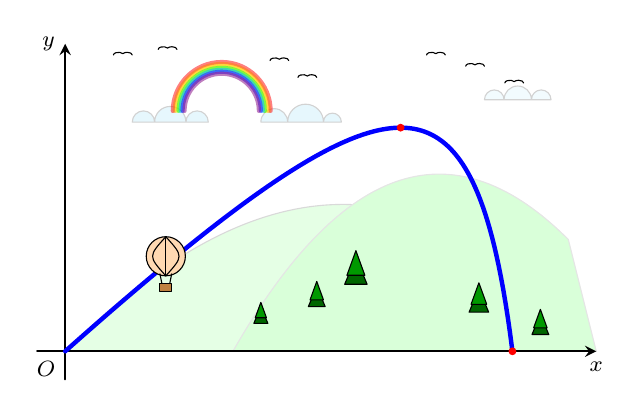
\begin{tikzpicture}[line cap=round, line join=round, >=stealth, font=\footnotesize, scale=0.71]
			% 1. Vẽ các dãy núi phía xa
			\draw[fill=green!10, draw=gray!30] (0,0) .. controls (2,2) and (4,3) .. (6,2.5) .. controls (8,2) and (9,1) .. (9.5,0) -- cycle;
			\draw[fill=green!15, draw=gray!20] (3,0) .. controls (5,3.5) and (7,4) .. (9,2) -- (9.5,0) -- cycle;
			
			% 2. Các đám mây làm điểm tựa cho cầu vồng
			% Đám mây bên trái (Điểm bắt đầu)
			\begin{scope}[shift={(1.2,4.1)}, scale=0.4, gray!35]
				\draw[fill=cyan!10] (0,0) arc (180:0:0.5) arc (180:0:0.7) arc (180:0:0.5) -- cycle;
			\end{scope}
			% Đám mây ở giữa (Điểm kết thúc cầu vồng)
			\begin{scope}[shift={(3.5,4.1)}, scale=0.4, gray!35]
				\draw[fill=cyan!10] (0,0) arc (180:0:0.6) arc (180:0:0.8) arc (180:0:0.4) -- cycle;
			\end{scope}
			% Đám mây thứ ba ở phía xa bên phải
			\begin{scope}[shift={(7.5,4.5)}, scale=0.35, gray!35]
				\draw[fill=cyan!5] (0,0) arc (180:0:0.5) arc (180:0:0.7) arc (180:0:0.5) -- cycle;
			\end{scope}
			
			% 3. Cầu vồng nối từ đám mây này sang đám mây kia
			\begin{scope}[shift={(2.8,4.3)}, opacity=0.5, scale=0.35]
				\foreach \c/\r in {red/2.5, orange/2.4, yellow/2.3, green/2.2, cyan/2.1, blue/2, violet/1.9}
				\draw[color=\c, line width=1.5pt] (\r,0) arc (0:180:\r); 
			\end{scope}
			
			% 4. Hàng cây thông đặt ở xa (phía trên Ox)
			\foreach \x/\y/\s in {4.5/0.8/0.3, 5.2/1.2/0.4, 3.5/0.5/0.25, 7.4/0.7/0.35, 8.5/0.3/0.3} {
				\begin{scope}[shift={(\x,\y)}, scale=\s]
					\draw[fill=green!40!black] (0,0) -- (0.5,0) -- (0,1.2) -- (-0.5,0) -- cycle;
					\draw[fill=green!60!black] (0,0.4) -- (0.4,0.4) -- (0,1.5) -- (-0.4,0.4) -- cycle;
				\end{scope}
			}
			
			% 5. Vẽ trục tọa độ
			\draw[->, thick] (-0.5,0) -- (9.5,0) node[below]{$x$};
			\draw[->, thick] (0,-0.5) -- (0,5.5) node[left]{$y$};
			\node[below left] at (0,0) {$O$};
			
			% 6. Hàm số y = (x^2 - 8x)/(x-9)
			\def\f{(\x)*(\x-8)/((\x)-9)}
			
			% 7. Chim bay rải rác
			\foreach \px/\py in {7.5/5.1, 8.2/4.8, 1.2/5.3, 2.0/5.4, 4.0/5.2, 4.5/4.9, 6.8/5.3} {
				\begin{scope}[shift={(\px,\py)}, scale=0.6]
					\draw (0,0) arc (0:150:0.15 and 0.08) arc (30:180:0.15 and 0.08);
				\end{scope}
			}
			
			% 8. Đường đi khinh khí cầu
			\draw[blue, ultra thick, samples=200, domain=0:8] plot(\x,{\f});
			
			% 9. Khinh khí cầu
			\begin{scope}[shift={(1.8,1.7)}, scale=0.35]
				\draw[fill=orange!30] (0,0) circle (1);
				\draw (-0.3,-0.9) -- (-0.2,-1.4) (0.3,-0.9) -- (0.2,-1.4);
				\draw[fill=brown] (-0.3,-1.4) rectangle (0.3,-1.8);
				\foreach \ang in {-45, 0, 45} \draw (0,1) .. controls (\ang/50,0) .. (0,-1);
			\end{scope}
			
			% 10. Các điểm đặc biệt
			\fill[red] (6,4) circle (2pt) node[above right, black, font=\boldmath]{};
			\fill[red] (8,0) circle (2pt) node[below right, black, font=\boldmath]{};
			%\draw[dashed, gray] (6,0) -- (6,4) -- (0,4);
	\end{tikzpicture}}
	\loigiai{
		Vì đồ thị cắt trục hoành tại $x=0$ và $x=8$ nên tử thức có dạng $a(x^2 - 8x)$. \\
		Khi đó: $f(x) = \dfrac{a(x^2 - 8x)}{x + d}$.
		
		Tại điểm cực trị $M(6;4)$, ta có giá trị cực trị bằng tỉ số đạo hàm tử và đạo hàm mẫu tại điểm đó:
		$$y_{ct} = \dfrac{(ax^2 - 8ax)'}{(x + d)'}\bigg|_{x=6} \Rightarrow 4 = \dfrac{2ax - 8a}{1} \bigg|_{x=6}$$
		$$\Leftrightarrow 4 = 12a - 8a \Leftrightarrow 4a = 4 \Leftrightarrow a = 1.$$
		
		Với $a=1$, thay tọa độ cực đại $(6;4)$ vào hàm số:
		$$4 = \dfrac{6^2 - 8 \cdot 6}{6 + d} \Leftrightarrow  d = -9.$$
		Do đó hàm số là $f(x) = \dfrac{x^2 - 8x}{x - 9}$.
		
		Khi khinh khí cầu cách mặt đất $2{,}5$ km, ta có:
		$$\dfrac{x^2 - 8x}{x - 9} = 2{,}5 \Leftrightarrow x^2 - 10{,}5x + 22{,}5 = 0 \Leftrightarrow \hoac{&x = 7{,}5 \\ &x = 3}$$
		
		Vì khinh khí cầu đang hạ cánh (sau khi qua điểm cực đại $x=6$), ta chọn $x = 7{,}5$ km.
		
		Vậy hình chiếu của khinh khí cầu trên trục $Ox$ cách gốc tọa độ $7{,}5$ km.
		
		
		\textit{Lưu ý:} Sau khi có  $f(x) = \dfrac{a(x^2 - 8x)}{x + d}$, ta cũng có thể giải bằng cách tính đạo hàm $f'(x)$, cho $f'(6)=0$ kết hợp với $f(6)=4$ để tìm hệ số $a, d$, tuy nhiên cách dùng công thức đạo hàm tử trên đạo hàm mẫu cho điểm cực trị sẽ nhanh gọn hơn.
		
		
		
	}
\end{ex}

\begin{ex}%Câu 3. %[2D4V3-5]
	\immini[thm]{Cho hình vuông $ABCD$ tâm $O$. Gọi $M, N, P, Q$ lần lượt là trung điểm của các đoạn $AB, BC, CD$ và $DA$. Các cung $\wideparen{QM}, \wideparen{MN}, \wideparen{NP}, \wideparen{PQ}$ lần lượt là các cung tròn của các đường tròn tâm $A, B, C, D$ với bán kính bằng nhau (tham khảo hình vẽ). Biết diện tích "tứ giác cong" $MNPQ$ (miền bị gạch chéo trong hình vẽ) bằng $25(4 - \pi)$ dm$^2$. Hỏi khi cho "tứ giác cong" $MNPQ$ quay quanh trục $NQ$ ta thu được vật thể có thể tích bằng bao nhiêu đềximét khối (kết quả làm tròn đến hàng phần mười)?
		\shortans[oly]{$75{,}3$}
	}{\begin{tikzpicture}[line cap=round, line join=round, >=stealth, font=\footnotesize, scale=1]
			% Tọa độ các đỉnh hình vuông
			\coordinate (B) at (0,4);
			\coordinate (A) at (4,4);
			\coordinate (D) at (4,0);
			\coordinate (C) at (0,0);
			\coordinate (O) at (2,2);
			
			% Tọa độ các trung điểm
			\coordinate (M) at (2,4);
			\coordinate (N) at (0,2);
			\coordinate (P) at (2,0);
			\coordinate (Q) at (4,2);
			
			% Tô màu miền "tứ giác cong" MNPQ bằng gạch chéo dựa trên ảnh gốc image_559363.png
			\begin{scope}
				\clip (2,4) arc (180:270:2) arc (90:180:2) arc (0:90:2) arc (270:360:2);
				\fill[pattern=north west lines, pattern color=cyan!80] (0,0) rectangle (4,4);
			\end{scope}
			
			% Vẽ các cạnh của hình vuông
			\draw[thick] (A)--(B)--(C)--(D)--cycle;
			
			% Vẽ 4 cung tròn chuẩn xác theo tâm A, B, C, D
			\draw[thick] (M) arc (180:270:2); % Cung QM tâm A
			\draw[thick] (N) arc (-90:0:2);   % Cung MN tâm B
			\draw[thick] (P) arc (0:90:2);   % Cung NP tâm C
			\draw[thick] (Q) arc (90:180:2); % Cung PQ tâm D
			
			% Vẽ các trục đối xứng NQ và MP (nối các trung điểm)
			\draw (N)--(Q);
			\draw (M)--(P);
			
			% Gán nhãn các điểm theo ảnh gốc
			\node[above right] at (A) {$A$};
			\node[above left] at (B) {$B$};
			\node[below left] at (C) {$C$};
			\node[below right] at (D) {$D$};
			\node[above] at (M) {$M$};
			\node[left] at (N) {$N$};
			\node[below] at (P) {$P$};
			\node[right] at (Q) {$Q$};
			\node[below right] at (O) {$O$};
			
			% Đánh dấu các điểm
			\foreach \p in {A,B,C,D,M,N,P,Q,O}
			\fill (\p) circle (1.5pt);
	\end{tikzpicture}}
	\loigiai{
		Gọi $R$ là bán kính các cung tròn (bằng nửa cạnh hình vuông). 
		Xét góc phần tư thứ nhất (hình vuông $MQOA$ cạnh $R$): \\
		Diện tích $\dfrac{1}{4}$ miền gạch chéo bằng diện tích hình vuông trừ đi diện tích hình quạt tròn tâm $A$:
		$$S_1 = R^2 - \dfrac{\pi R^2}{4} = \dfrac{R^2}{4}(4 - \pi).$$
		Do tính đối xứng, diện tích miền $MNPQ$ là $S = 4S_1 = R^2(4 - \pi)$. \\
		Theo giả thiết: $R^2(4 - \pi) = 25(4 - \pi) \Rightarrow R = 5$ (dm). 
		
		Chọn hệ trục tọa độ $Oxy$ với $O(0;0)$, trục $Ox$ trùng với $NQ$, trục $Oy$ trùng với $MP$. 
		\begin{center}
			\begin{tikzpicture}[line cap=round, line join=round, >=stealth, font=\footnotesize, scale=0.8]
				% Vẽ hệ trục tọa độ Oxy tại tâm O
				\draw[->] (-3.5,0) -- (4.8,0) node[below]{$x$};
				\draw[->] (0,-3.5) -- (0,3.8) node[left]{$y$};
				\node[below left] at (0,0) {$O$};
				
				% Tọa độ các đỉnh (R=2.5 để hình gọn hơn trong LaTeX)
				\coordinate (A) at (2.5,2.5);
				\coordinate (B) at (-2.5,2.5);
				\coordinate (C) at (-2.5,-2.5);
				\coordinate (D) at (2.5,-2.5);
				\coordinate (M) at (0,2.5);
				\coordinate (N) at (-2.5,0);
				\coordinate (P) at (0,-2.5);
				\coordinate (Q) at (2.5,0);
				
				% Tô màu miền tứ giác cong
				\begin{scope}
					\clip (0,2.5) arc (180:270:2.5) arc (90:180:2.5) arc (0:90:2.5) arc (270:360:2.5);
					\fill[pattern=north west lines, pattern color=cyan!60] (-2.5,-2.5) rectangle (2.5,2.5);
				\end{scope}
				
				% Vẽ các cung tròn và hình vuông
				\draw[thick] (A)--(B)--(C)--(D)--cycle;
				\draw[thick, red] (M) arc (180:270:2.5); % Cung MQ tâm A
				\draw[thick, blue] (N) arc (-90:0:2.5);  % Cung MN tâm B
				\draw[thick, blue] (P) arc (0:90:2.5);   % Cung NP tâm C
				\draw[thick, blue] (Q) arc (90:180:2.5); % Cung PQ tâm D
				
				% Gán nhãn tọa độ điểm đặc biệt
				\node[above right] at (A) {$A(5;5)$};
				\node[above left] at (M) {$M$};
				\node[below right] at (Q) {$Q(5;0)$};
				\node[below left] at (N) {$N(-5;0)$};
				
				\foreach \p in {A,B,C,D,M,N,P,Q,O} \fill (\p) circle (1.5pt);
			\end{tikzpicture}
		\end{center}
		Cung tròn $\wideparen{MQ}$ là một phần của đường tròn tâm $A(5; 5)$ bán kính $R=5$. \\
		Phương trình đường tròn tâm $A$ là: $(x-5)^2 + (y-5)^2 = 25$. \\
		Từ đó ta có phương trình cung $\wideparen{MQ}$: $y = 5 - \sqrt{25 - (x - 5)^2}$ với $x \in [0; 5]$. 
		
		Do tính đối xứng, thể tích vật thể bằng 2 lần thể tích tạo bởi miền bên phải trục $Oy$ ($x \in [0; 5]$) nằm trên trục $Ox$ quay quanh $Ox$:
		$$V = 2 \cdot \pi \displaystyle\int_{0}^{5} \left( 5 - \sqrt{25 - (x-5)^2} \right)^2 \mathrm{d}x \approx 75{,}3  (\text{dm}^3).$$
		
	}
\end{ex}
\begin{ex}%Câu 4. %[1D6V3-5]
	Hai cột điện $AC, BD$ dựng vuông góc với mặt đất và cách nhau $100$ mét ($AB = CD = 100$ mét). Một dây điện được treo từ đầu $A$ cột này đến đầu $B$ cột kia (tham khảo hình vẽ) với $AC = BD$. Chọn hệ tọa độ $Oxy$ sao cho tia $Ox$ trùng với tia $OD$ ($O$ là trung điểm $CD$), tia $Oy$ cùng hướng với tia $CA$, mỗi đơn vị trên các trục là $1$ mét. Khi đó, người ta thấy rằng dây điện nằm trong mặt phẳng $Oxy$ và tạo thành một đường cong catenary có phương trình $y = 202 \left( \mathrm{e}^{\tfrac{x}{404}} + \mathrm{e}^{-\tfrac{x}{404}} \right) - 386$, với $-50 \le x \le 50$.
	Gọi khoảng cách từ điểm thấp nhất trên dây điện đến đường thẳng nằm ngang $AB$ là độ võng của dây điện. Hỏi độ võng của dây điện bằng bao nhiêu mét (kết quả làm tròn đến hàng phần mười)?
	\shortans[oly]{$3{,}1$}
	\vspace{-2cm}
	\begin{center}
		
		\begin{tikzpicture}[line cap=round, line join=round, >=stealth, font=\footnotesize, scale=0.066]
			% Khai báo các tham số dựa trên đề bài
			\def\xmin{-70} \def\xmax{70}
			\def\ymin{-20} \def\ymax{40}
			
			% Tọa độ các điểm chính (đơn vị mét)
			% C(-50,0), D(50,0), O(0,0)
			% A(-50, y(-50)), B(50, y(50))
			\pgfmathsetmacro{\yA}{202*(exp(-50/404) + exp(50/404)) - 386}
			\coordinate (C) at (-50,0);
			\coordinate (D) at (50,0);
			\coordinate (O) at (0,0);
			\coordinate (A) at (-50,\yA);
			\coordinate (B) at (50,\yA);
			
			% Vẽ mặt đất (trục Ox)
			\draw[] (\xmin,0) -- (\xmax,0) node[right] {};
			%			\draw[->] (0,\ymin) -- (0,\ymax) node[above] {$y$};
			
			% Vẽ cột điện AC và BD
			\draw[ultra thick] (C) -- (A) node[midway, left, xshift=-2pt] {cột điện};
			\draw[ultra thick] (D) -- (B) node[midway, right, xshift=2pt] {cột điện};
			
			% Vẽ dây điện (đường cong catenary)
			\begin{scope}
				\clip (\xmin,\ymin) rectangle (\xmax,\ymax+10);
				\draw[blue, thick, smooth, samples=100, domain=-50:50] 
				plot(\x, {202*(exp(\x/404) + exp(-\x/404)) - 386});
			\end{scope}
			
			% Vẽ đường nằm ngang AB (nối hai đầu cột)
			\draw[dashed] (A) -- (B);
			
			% Ghi chú các điểm
			\fill (A) circle (30pt) node[above left] {$A$};
			\fill (B) circle (30pt) node[above right] {$B$};
			\fill (C) circle (30pt) node[below] {$C$};
			\fill (D) circle (30pt) node[below] {$D$};
			\fill (O) circle (30pt) node[below right] {$O$};
			
			% Kích thước khoảng cách giữa 2 cột
			%			\draw[<->] (-50,-10) -- (50,-10) node[midway, fill=white] {100 m};
			
			% Nhãn mô tả dây điện
			\node[below] at (0, 18) {dây điện};
			
			% Thể hiện độ võng (khoảng cách từ đỉnh AB xuống điểm thấp nhất của dây)
			\pgfmathsetmacro{\yMin}{202*(exp(0) + exp(0)) - 386} % y(0) = 202*2 - 386 = 18
			%			\draw[<->, red] (0,\yMin) -- (0,\yA) node[midway, right] {$d$};
		\end{tikzpicture}
	\end{center}
	\loigiai{
		\begin{center}
			
			\begin{tikzpicture}[line cap=round, line join=round, >=stealth, font=\footnotesize, scale=0.08]
				
				% Khai báo các tham số dựa trên đề bài
				\def\xmin{-70} \def\xmax{70}
				\def\ymin{-20} \def\ymax{40}
				
				% Tọa độ các điểm chính (đơn vị mét)
				% C(-50,0), D(50,0), O(0,0)
				% A(-50, y(-50)), B(50, y(50))
				\pgfmathsetmacro{\yA}{202*(exp(-50/404) + exp(50/404)) - 386}
				\coordinate (C) at (-50,0);
				\coordinate (D) at (50,0);
				\coordinate (O) at (0,0);
				\coordinate (A) at (-50,\yA);
				\coordinate (B) at (50,\yA);
				
				% Vẽ mặt đất (trục Ox)
				\draw[->] (\xmin,0) -- (\xmax,0) node[right] {$x$};
				\draw[->] (0,\ymin) -- (0,\ymax) node[above] {$y$};
				
				% Vẽ cột điện AC và BD
				\draw[ultra thick] (C) -- (A) node[midway, left, xshift=-2pt] {cột điện};
				\draw[ultra thick] (D) -- (B) node[midway, right, xshift=2pt] {cột điện};
				
				% Vẽ dây điện (đường cong catenary)
				\begin{scope}
					\clip (\xmin,\ymin) rectangle (\xmax,\ymax+10);
					\draw[blue, thick, smooth, samples=100, domain=-50:50] 
					plot(\x, {202*(exp(\x/404) + exp(-\x/404)) - 386});
				\end{scope}
				
				% Vẽ đường nằm ngang AB (nối hai đầu cột)
				\draw[dashed] (A) -- (B);
				
				% Ghi chú các điểm
				\fill (A) circle (30pt) node[above left] {$A$};
				\fill (B) circle (30pt) node[above right] {$B$};
				\fill (C) circle (30pt) node[below] {$C$};
				\fill (D) circle (30pt) node[below] {$D$};
				\fill (O) circle (30pt) node[below right] {$O$};
				
				% Kích thước khoảng cách giữa 2 cột
				\draw[<->] (-50,-10) -- (50,-10) node[midway, fill=white] {100 m};
				
				% Nhãn mô tả dây điện
				\node[below] at (0, 18) {dây điện};
				
				% Thể hiện độ võng (khoảng cách từ đỉnh AB xuống điểm thấp nhất của dây)
				\pgfmathsetmacro{\yMin}{202*(exp(0) + exp(0)) - 386} % y(0) = 202*2 - 386 = 18
				\draw[<->, red] (0,\yMin) -- (0,\yA) node[midway, right] {$d$};
				
			\end{tikzpicture}
		\end{center}
		Vì $O$ là trung điểm của $CD$ và $CD = 100$ m nên tọa độ của điểm $C$ và $D$ lần lượt là $C(-50; 0)$ và $D(50; 0)$.
		
		Chiều cao của cột điện chính là tung độ của điểm $A$ (hoặc $B$). Với $x = 50$, ta có:
		$$y_A = y_B = 202 \left( \mathrm{e}^{\tfrac{50}{404}} + \mathrm{e}^{-\tfrac{50}{404}} \right) - 386\approx 21{,}09801... \text{ (m)}.$$
		
		Điểm thấp nhất của dây điện nằm tại đỉnh của đường cong catenary, tương ứng với $x = 0$ (do tính đối xứng):
		$$y_{min} = y(0) = 202 \left( \mathrm{e}^0 + \mathrm{e}^0 \right) - 386 = 18 \text{ (m)}.$$
		
		Độ võng của dây điện là khoảng cách từ điểm thấp nhất đến đường thẳng $AB$ (đường thẳng nối hai đầu cột $y = y_A$):
		$$d = y_A - y_{min}  \approx 3{,}1 \text{ (m)}.$$
		
		
		
	}
\end{ex}

\begin{ex}%Câu 5. %[2H5C3-8]
	Trong không gian $Oxyz$, cho mặt phẳng $(P) \colon y - 1 = 0$, đường thẳng $d \colon \heva{&x = 1 \\ &y = 2 - t \\ &z = 1}$ và hai điểm $A(-1; -3; 11)$, $B\left(\dfrac{1}{2}; 0; 8\right)$. Hai điểm $M, N$ thuộc mặt phẳng $(P)$ sao cho $M$ luôn cách đường thẳng $d$ một khoảng bằng $2$ và $NA = 2NB$. Khoảng cách nhỏ nhất giữa hai điểm $M$ và $N$ bằng bao nhiêu?
	\shortans[oly]{$1$}
	\loigiai{
		
		Mặt phẳng $(P)$ có VTPT $\vec{n}_P = (0; 1; 0)$, đường thẳng $d$ có VTCP $\vec{u}_d = (0; -1; 0)$. 
		
		Nhận thấy $\vec{u}_d$ cùng phương với $\vec{n}_P$ nên $d \perp (P)$. 
		
		Giao điểm của $d$ và $(P)$ là $I_1(1; 1; 1)$. 
		Vì $d \perp (P)$ tại $I_1$ nên khoảng cách từ $M \in (P)$ đến $d$ chính là đoạn $MI_1 = 2$. 
		
		Do đó tập hợp các điểm $M$ là đường tròn $(C_1)$ tâm $I_1(1; 1; 1)$, bán kính $R_1 = 2$ nằm trong $(P)$.
		
		
		Điểm $N \in (P)$ nên $N(x; 1; z)$. Từ $NA = 2NB \Leftrightarrow NA^2 = 4NB^2$
		$$\Leftrightarrow(x+1)^2 + (1+3)^2 + (z-11)^2 = 4\left[\left(x-\dfrac{1}{2}\right)^2 + (1-0)^2 + (z-8)^2\right]$$
		$$\Leftrightarrow 3x^2 - 6x + 3z^2 - 42z + 123 = 0 \Leftrightarrow (x-1)^2 + (z-7)^2 = 9.$$
		Do đó $N$ thuộc đường tròn $(C_2)$ tâm $I_2(1; 1; 7)$, bán kính $R_2 = 3$.
		
		
		\begin{center}
			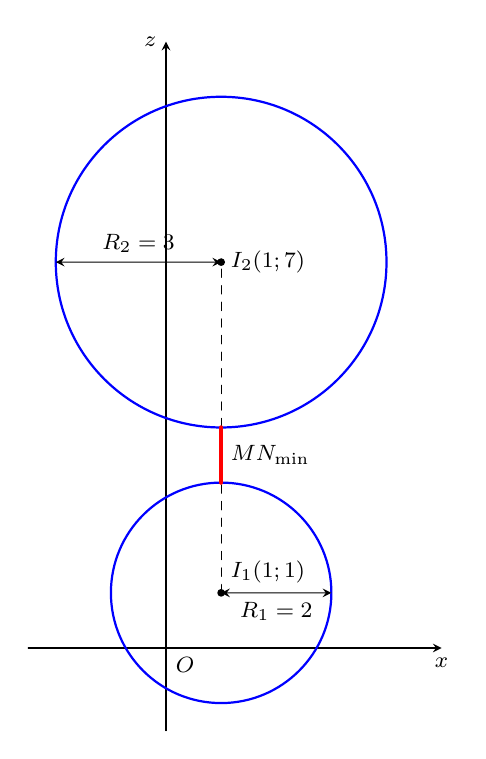
\begin{tikzpicture}[scale=0.7, font=\footnotesize, line join=round, line cap=round, >=stealth]
				% Vẽ hệ trục tọa độ trong mặt phẳng y=1 (chỉ vẽ Ox, Oz để minh họa)
				\draw[->] (-2.5,0) -- (5,0) node[below] {$x$};
				\draw[->] (0,-1.5) -- (0,11) node[left] {$z$};
				\node[below right] at (0,0) {$O$};
				
				% Vẽ đường tròn C1
				\coordinate (I1) at (1,1);
				\draw[thick, blue] (I1) circle (2);
				\fill (I1) circle (2pt) node[above right] {$I_1(1;1)$};
				
				% Vẽ đường tròn C2
				\coordinate (I2) at (1,7);
				\draw[thick, blue] (I2) circle (3);
				\fill (I2) circle (2pt) node[right] {$I_2(1;7)$};
				
				% Vẽ đoạn nối tâm và khoảng cách MN min
				\draw[dashed] (I1) -- (I2);
				\draw[ultra thick, red] (1,3) -- (1,4);
				\node[right] at (1,3.5) {$MN_{\min}$};
				
				% Ký hiệu bán kính
				\draw[<->] (I1) -- (3,1) node[midway, below] {$R_1=2$};
				\draw[<->] (I2) -- (-2,7) node[midway, above] {$R_2=3$};
			\end{tikzpicture}
		\end{center}
		Cả $M$ và $N$ cùng nằm trong mặt phẳng $y=1$. 
		
		Khoảng cách giữa hai tâm: 			
		$I_1I_2 = \sqrt{(1-1)^2 + (1-1)^2 + (7-1)^2} = 6$.
		
		Khoảng cách nhỏ nhất giữa hai điểm $M$ và $N$ là:
		
		$$MN_{\min} = I_1I_2 - R_1 - R_2 = 6 - 2 - 3 = 1.$$
		
	}
\end{ex}

\begin{ex}%Câu 6. %[1D6C1-1]
	Chọn ngẫu nhiên cặp số bất kì $(x; y)$ thỏa mãn $x, y$ thuộc tập hợp\\ $\{2008^1; 2008^2; 2008^3; \dots; 2008^{24}; 2008^{25}\}$. Xét biến cố $A \colon$ "$\log_x y$ có giá trị là một số nguyên". Biết rằng xác suất của biến cố $A$ bằng $\dfrac{a}{b}$ (với $a, b$ là các số nguyên dương, phân số $\dfrac{a}{b}$ tối giản). Tổng $a + b$ bằng bao nhiêu?
	\shortans[oly]{$712$}
	\loigiai{
		Số phần tử của tập hợp là $25$.
		
		Số phần tử của không gian mẫu khi chọn cặp $(x; y)$ là: $n(\Omega) = 25 \cdot 25 = 625$.
		
		Giả sử $x = 2008^m$ và $y = 2008^n$ với $m, n \in \{1; 2; \dots; 25\}$.
		
		Ta có $\log_x y = \log_{2008^m} (2008^n) = \dfrac{n}{m}$.
		
		Để $\log_x y$ là một số nguyên thì $n$ phải là bội của $m$ ($n = k \cdot m$ với $k \in \mathbb{Z}^+$).
		
		Ta đếm số cặp $(m; n)$ thỏa mãn bằng cách liệt kê theo $m$:
		\begin{center}
			\begin{tabular}{|c|l|c|}
				\hline
				$m$ & Các giá trị của $n$ (bội của $m$ không vượt quá $25$) & Số lượng \\ \hline
				$1$ & $1, 2, 3, \dots, 25$ & $25$ \\ \hline
				$2$ & $2, 4, 6, \dots, 24$ & $12$ \\ \hline
				$3$ & $3, 6, 9, \dots, 24$ & $8$ \\ \hline
				$4$ & $4, 8, 12, 16, 20, 24$ & $6$ \\ \hline
				$5$ & $5, 10, 15, 20, 25$ & $5$ \\ \hline
				$6$ & $6, 12, 18, 24$ & $4$ \\ \hline
				$7$ & $7, 14, 21$ & $3$ \\ \hline
				$8$ & $8, 16, 24$ & $3$ \\ \hline
				$9 \to 12$ & Mỗi số có $2$ bội (ví dụ $9, 18$; $10, 20$; ...) & $4 \times 2 = 8$ \\ \hline
				$13 \to 25$ & Mỗi số có đúng $1$ bội là chính nó & $13 \times 1 = 13$ \\ \hline
				\multicolumn{2}{|c|}{\textbf{Tổng cộng}} & \textbf{87} \\ \hline
			\end{tabular}
		\end{center}
		
		Số kết quả thuận lợi cho biến cố $A$ là $n(A) = 87$.
		
		Xác suất của biến cố $A$ là: $P(A) = \dfrac{87}{625}$.
		
		Vậy $a + b = 87 + 625 = 712$.
		
		
		\begin{luuy}
			Tổng quát, số kết quả thuận lợi $n(A)$ có thể tính nhanh bằng công thức dùng hàm phần nguyên:
			$$n(A) = \sum_{x=1}^{25} \left\lfloor \dfrac{25}{x} \right\rfloor=87$$
			với $\lfloor x \rfloor$ là phần nguyên của $x$.
		\end{luuy}
	}
\end{ex}

\Closesolutionfile{ans}

\indapan{6}{ans/ans 57-26-2--BacNinh-SoGD-L1-LC}
\indapan{4}{ans/ans 57-26-2--BacNinh-SoGD-L1-DS}
\indapan{6}{ans/ans 57-26-2--BacNinh-SoGD-L1-KQ}
